\documentclass[12pt]{article}

\usepackage{times}
\usepackage{textcomp}
\usepackage{listings}
\usepackage{fullpage}
\usepackage{color}
\usepackage{hyperref} 
\usepackage{pst-tree} 
\usepackage{verbatim} 
\usepackage{graphicx}
\usepackage{amsmath,amsfonts,amssymb,amsthm}
\graphicspath{ {./}}


\def\part#1{\item[\bf #1)]}
\renewcommand{\thesubsection}{Question \arabic{subsection}}

\author{Clement Tsang}

\begin{document}

\begin{center}
    \Large\textbf{CS 241, Lecture 14 - SLR(1) and LR(1) Parsers}
\end{center}

\section{Bottom-up Parsing}
\begin{itemize}
    \item Knuth defines a theorem, that the set $\{wa: \exists x s.t. S \Rightarrow^* wax\}$, where $w$ is the stack and $a$ is the next character in a regular language.
    \item Note that this is actually a DFA that also writes output - these are called finite state transducers.
    \item Let us construct an LR(0) DFA with the following grammar:
        \begin{align*}
            &S' \rightarrow \vdash S \dashv \\
            &S \rightarrow S + T \\
            &S \rightarrow T \\
            &T \rightarrow d
        \end{align*}
    \item From each state, for each rule, we move a ``dot'' forward by one character.  For example, with $S' \rightarrow \cdot \vdash S \dashv$, we move the $\cdot$ over $\vdash$.  The transition function consumes the $vdash$.
    \item This leaves us with $S' \rightarrow \vdash \cdot S \dashv$.  This state would also have $S \rightarrow \cdot S + T$ and $S \rightarrow \cdot T$.  
    \item We also need to consider, now, $T \rightarrow \cdot d$.
    \item We are left with the following LR(0) grammar:\\
        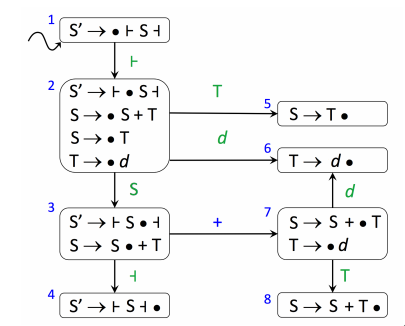
\includegraphics[scale=0.7]{LRgrammar1.png}
    \item To use this automation, start in a start state with an empty stack. Either:
        \begin{itemize}
            \item Shift: shift a character from input to the stack.  Follow any transition that follows with the character as a label; if none, reduce or if not possible, give an error.
            \item Reduce: reduce states that only have one item and the $\cdot$ is in the rightmost position.  Pop the RHS off the stack and backtrack in your DFA the number of states corresponding to the number of elements in the RHS.  Follow the transition for the LHS and push the LHS on the stack.
        \end{itemize}
    \item Accept if $S'$ is on the stack and the index is empty.
    \item For example, for string $\vdash d + d + d \dashv$: \\
        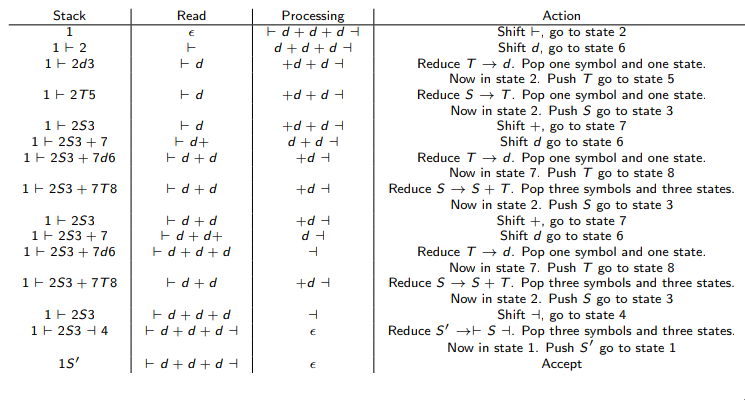
\includegraphics[scale=0.5]{lrauto.png}
    \item This, however, leaves issues on whether we should shift or reduce (shift-reduce) or \emph{which} item to reduce (reduce-reduce).
    \item We take the sledgehammer approach - ignore all grammars that have these problems!
    \item We say a grammar is LR(0) iff after creating the Knuth transducer, no state has these conflicts!
    \item We see that, like how LL(1) grammars were never left recursive, that LR(0) grammars are never right associative.  For example, this grammar:
        \begin{align*}
            &S' \rightarrow \vdash S \dashv \\
            &S \rightarrow T + S \\
            &S \rightarrow T \\
            &T \rightarrow d
        \end{align*}
    \item Observe the following resulting LR(0) automation:\\
        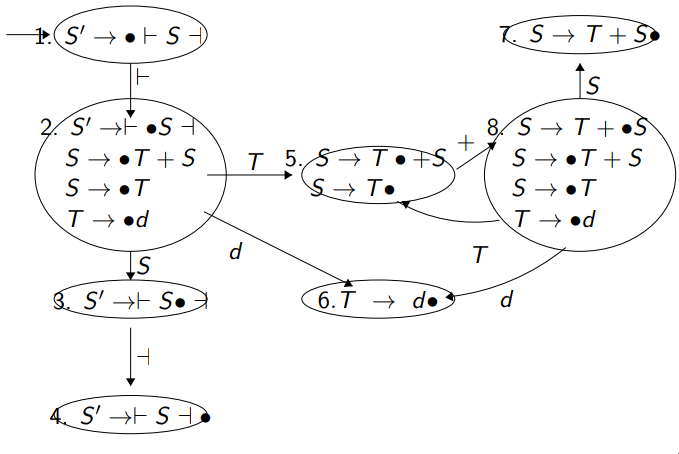
\includegraphics[scale=0.5]{conflict.png}\\
        We see that state 5 has a shift-reduce conflict.  We can fix this if our input instead began with $\vdash d$.  This would give us a stack of $\vdash d$ which we reduce in state 6, so our stack changes from $\vdash T$ to state 5 via state 1. 
    \item But this still gives a problem... we may want to reduce $S \rightarrow T$ depending on if the input is $\vdash d \dashv$ or $\vdash d + \dots$ (no to the latter).
    \item We fix this with a lookahead.  For every $A \rightarrow \alpha \cdot$, attach Follow($A$).  We also do this for $S$ and $T$.  So, state 5 would become $S \rightarrow T \cdot + S$ and $S \rightarrow T \cdot \{\dashv\}$.  That is, apply the first rule if the next token is $+$ and apply the second rule if the next token is $\dashv$.
    \item We call these parsers SLR(1) parsers - simple LR with 1 char. lookahead.
    \item There exist LR(1) parsers, but instead of adding all of Follow($S$) to an item, we add a subset of this set to each item.
    \item The algorithm for a LR(1) DFA is as follows, for $S_M$ being a set of states of a DFA $M$:\\
        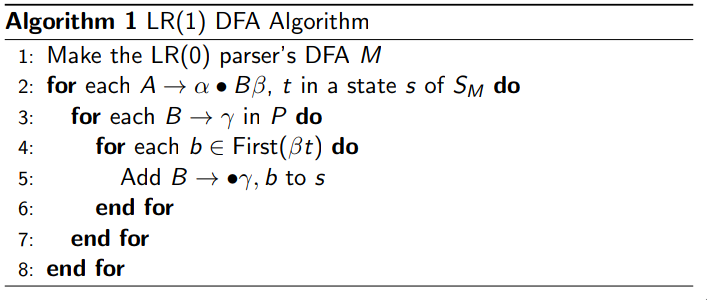
\includegraphics[scale=0.5]{lr1alg.png}
    \item Consider a sample LR(1) grammar that is \textbf{not} SLR(1):
        \begin{align*}
            &S \rightarrow aA\\
            &S \rightarrow bAc\\
            &S \rightarrow dc\\
            &S \rightarrow bda\\
            &A \rightarrow d
        \end{align*}
    This gives a SLR(1) table as such:\\
    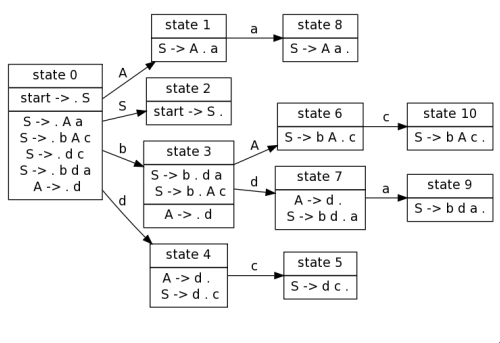
\includegraphics[scale=0.5]{slrfalsetable.png}\\
    It also gives the SLR(1) table:\\
    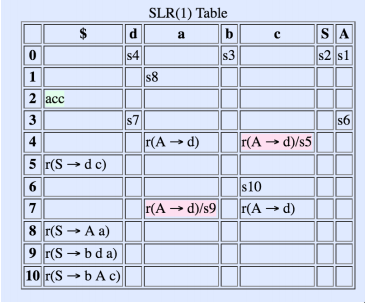
\includegraphics[scale=0.5]{slr1table.png}\\
    Meanwhile, the LR(1) table is:\\
    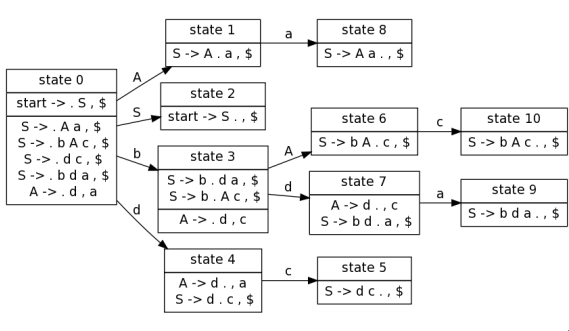
\includegraphics[scale=0.5]{lr1falsetable.png}\\
    Its accompanying LR(1) table:\\
    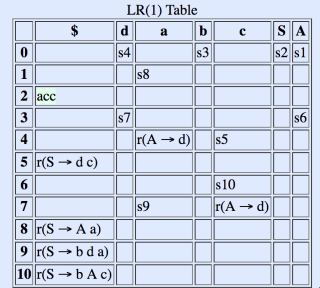
\includegraphics[scale=0.5]{lr1table.png}
\end{itemize}

\end{document}

